\documentclass[final]{beamer}

\usepackage[scale=1.24]{beamerposter} % Use the beamerposter package for laying out the poster

\usetheme{epyt} % Use the confposter theme supplied with this template

\setbeamercolor{block title}{fg=ngreen,bg=white} % Colors of the block titles
\setbeamercolor{block body}{fg=black,bg=white} % Colors of the body of blocks
\setbeamercolor{block alerted title}{fg=white,bg=dblue!70} % Colors of the highlighted block titles
\setbeamercolor{block alerted body}{fg=black,bg=dblue!10} % Colors of the body of highlighted blocks

\newlength{\sepwid}
\newlength{\onecolwid}
\newlength{\twocolwid}
\newlength{\threecolwid}
\setlength{\paperwidth}{48in} % A0 width: 46.8in
\setlength{\paperheight}{36in} % A0 height: 33.1in
\setlength{\sepwid}{0.024\paperwidth} % Separation width (white space) between columns
\setlength{\onecolwid}{0.22\paperwidth} % Width of one column
\setlength{\twocolwid}{0.464\paperwidth} % Width of two columns
\setlength{\threecolwid}{0.708\paperwidth} % Width of three columns
\setlength{\topmargin}{-0.5in} % Reduce the top margin size
%-----------------------------------------------------------

\usepackage{graphicx}  % Required for including images

\usepackage{booktabs} % Top and bottom rules for tables

\title{Project: Image classification using CIFAR-10}

\author{Sascha Stelling}




%----------------------------------------------------------------------------------------

\begin{document}
	
\addtobeamertemplate{block end}{}{\vspace*{2ex}} % White space under blocks
\addtobeamertemplate{block alerted end}{}{\vspace*{2ex}} % White space under highlighted (alert) blocks


\setlength{\belowcaptionskip}{2ex} % White space under figures
\setlength\belowdisplayshortskip{2ex} % White space under equations


\begin{frame} % The whole poster is enclosed in one beamer frame

\begin{columns} % The whole poster consists of three major columns, the second of which is split into two columns twice - the [t] option aligns each column's content to the top

\begin{column}{\sepwid}\end{column} % Empty spacer column

\begin{column}{\onecolwid} % The first column

\begin{alertblock}{Motivation}
\begin{itemize}
	\item Classify images using HoG features and SVM
	\item Classify again using CNN and softmax
	\item Classify again using CNN and SVM
	\item Compare results
\end{itemize}

\end{alertblock}



\begin{block}{Dataset: CIFAR-10}
	\begin{itemize}
		\item Labeled subset of the 80 million tiny images dataset
		\item Contains 60.000 color images of size 32x32
		\item Images are labeled as one out of 10 classes
		\item Each class contains 6.000 images
		\item 50.000 training and 10.000 test images
	\end{itemize}
\end{block}

\begin{block}{Classification method}
	\begin{itemize}
		\item HoG and SVM
		\begin{itemize}
			\item Compute HoG features and let SVM classify them
			\item SVM one vs all approach with linear kernel 
		\end{itemize}
		\item CNN with Softmax
		\begin{itemize}
			\item Let CNN learn the features by itself and use Softmax loss function for classification 
		\end{itemize}
		\item CNN with SVM
		\begin{itemize}
			\item Let CNN learn the features and use SVM for classification
		\end{itemize}
	\end{itemize}
\end{block}

\begin{block}{Results}
	Some images and their computation results
	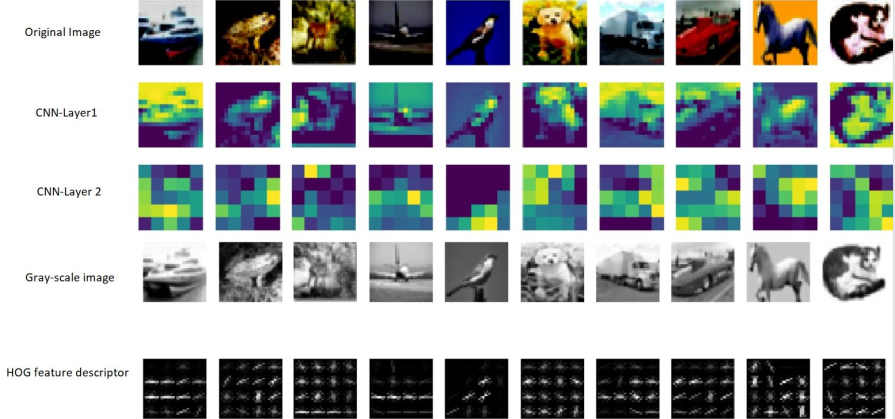
\includegraphics[width=\linewidth]{imgs}
\end{block}

\begin{block}{Results}
	Classification example
	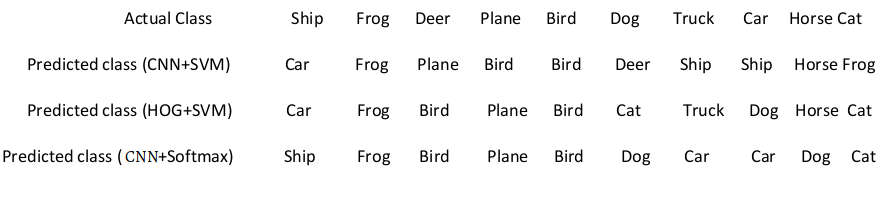
\includegraphics[width=\linewidth]{pics}
	
	
	Accuracies
	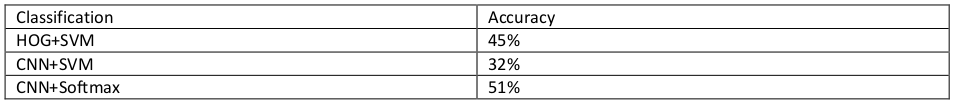
\includegraphics[width=\linewidth]{table}
\end{block}

\begin{block}{Evaluation}
	\begin{itemize}
		\item CNN+Softmax was expected to get the highest accuracy since it is a commonly used approach
		\item CNN+SVM would be expected to get higher accuracy than HoG+SVM
		\item HoG features seem to be better feature descriptor than simply learning them 
	\end{itemize}
\end{block}

\end{frame}
\end{document}